% CHAPTER 8: Cross-attention
\chapter{Cross-Attention}

Earlier on, we studied about an attention mechanism called \textbf{self-attention}. In this chapter, we will focus on another attention mechanism called \textbf{cross-attention}. At its core, cross attention is a mechanism that enables a model to focus on relevant information from one sequence while processing another sequence. Unlike self-attention, where a model attends to tokens within the same sequence, cross attention involves querying one sequence (e.g., decoder input) using another sequence’s representations (e.g., encoder output).
\begin{figure}[H]
    \centering
    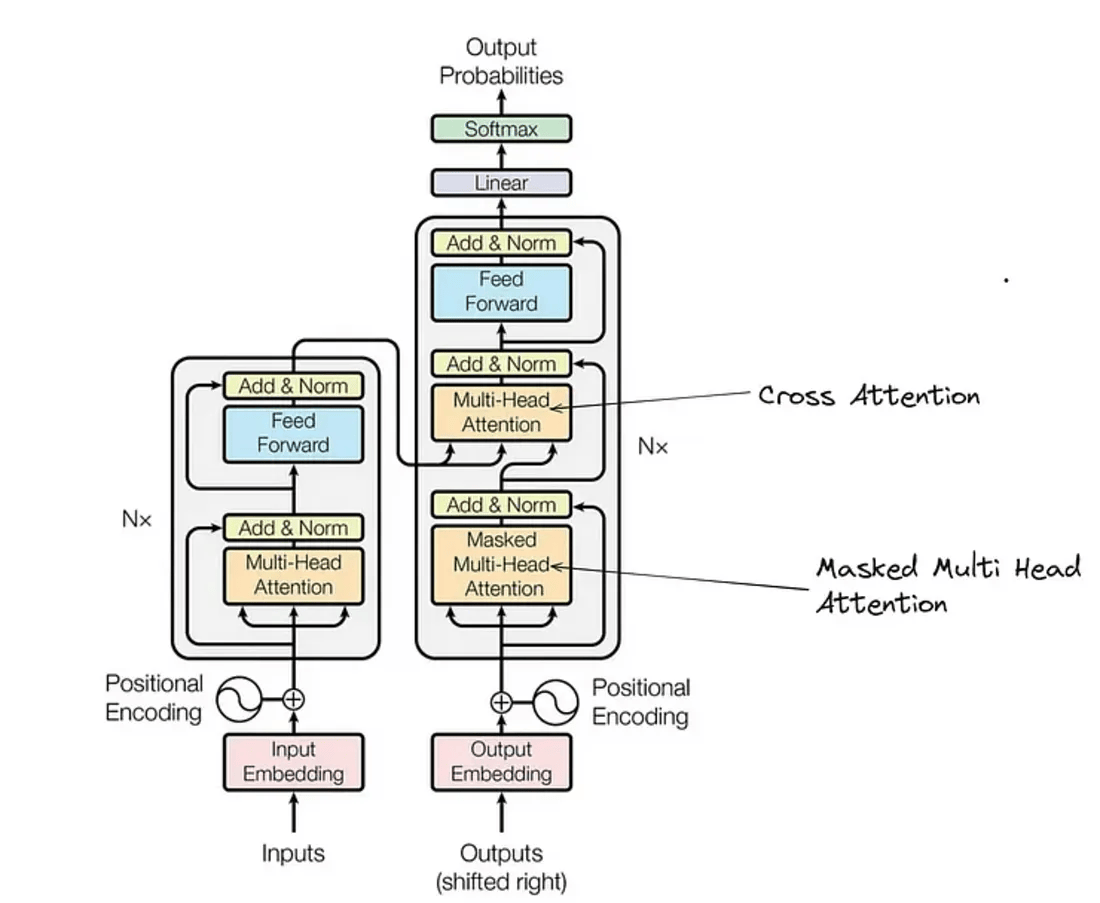
\includegraphics[width=0.5\linewidth]{Cross-Attention/architecture-cross-attention.png}
    \caption{Cross-attention architecture}
\end{figure}

% Why cross-attention
\section{Why is cross-attention necessary?}

Imagine that we are converting an English sentence \textit{“I like eating ice cream”} into Hindi. This process typically involves an encoder-decoder setup. The encoder reads the input sentence and understands its context, while the decoder generates the corresponding output in Hindi, step by step.
\begin{figure}[H]
    \centering
    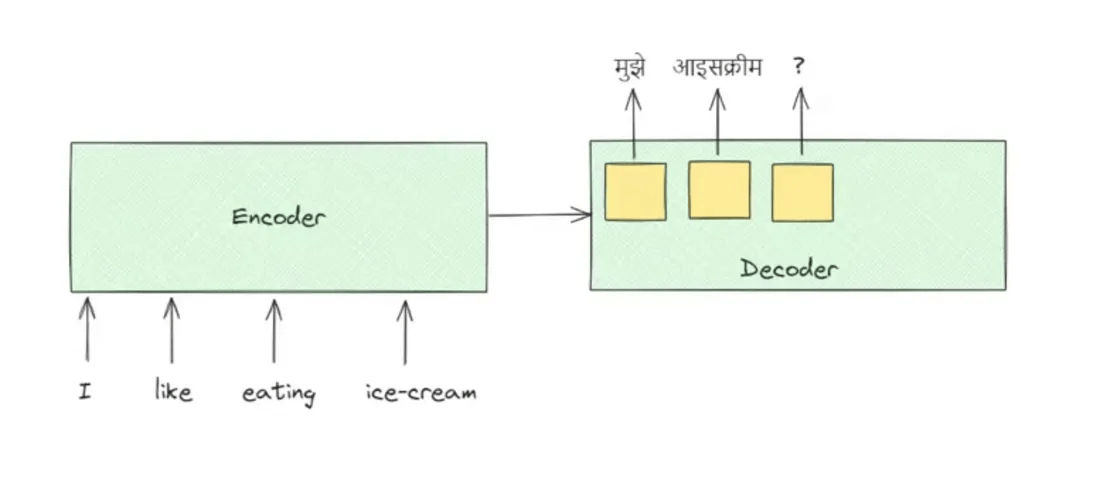
\includegraphics[width=0.7\linewidth]{Cross-Attention/encoder-decoder-translation.png}
    \caption{Translation by transformer}
\end{figure}

At each step, the decoder needs to generate the next word. For instance, after generating 
{\devanagarifont मुझे} and {\devanagarifont आइसक्रीम}, the decoder needs to figure out the next word, which in this case would be {\devanagarifont खाना} (eating). But how does the decoder decide this? It depends on two key factors:
\begin{enumerate}
    \item What has been generated so far, i.e., {\devanagarifont मुझे} and {\devanagarifont आइसक्रीम}.
    \item The input sentence itself, meaning the information passed from the encoder.
\end{enumerate}

To handle the first factor, self-attention is used, which helps the decoder understand how previously generated words relate to each other. For the second factor - understanding the relationship between the input sentence and the output sentence - cross attention comes into play. It allows the decoder to determine how words in the input sequence (e.g., “ice cream”) relate to words in the output sequence (e.g., {\devanagarifont “आइसक्रीम”}). The below figure demonstrates this, where the larger circles demonstrate stronger relationship.
\begin{figure}[H]
    \centering
    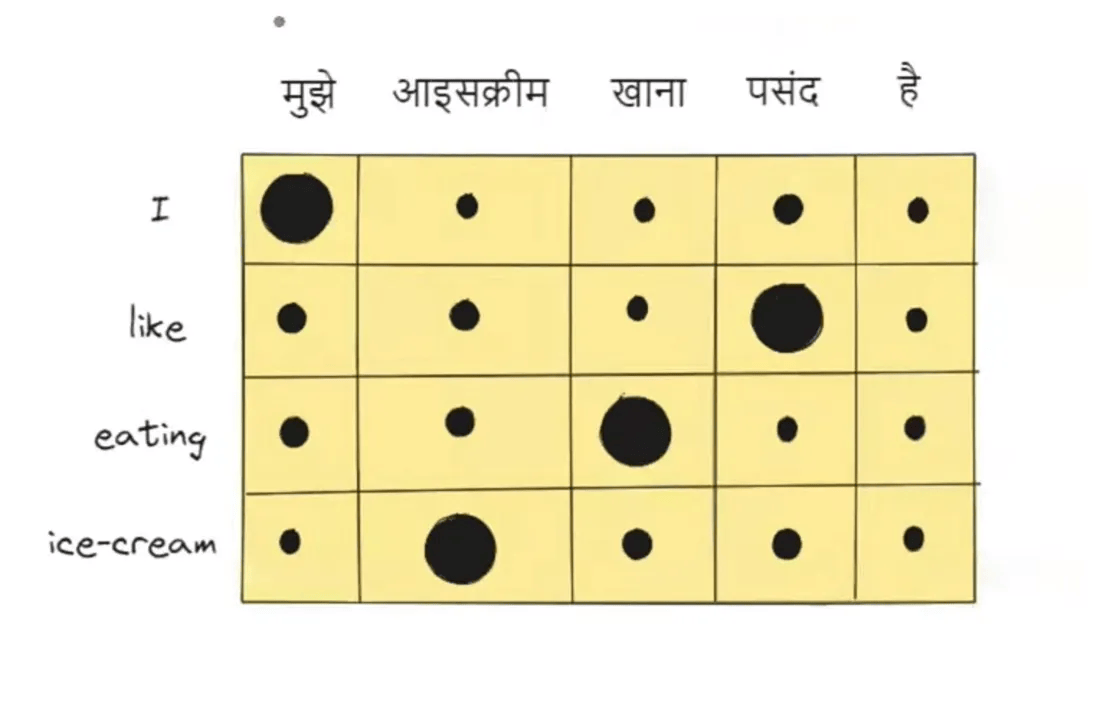
\includegraphics[width=0.5\linewidth]{Cross-Attention/cross-attention-matrix.png}
    \caption{Cross-attention matrix between 2 sequences}
\end{figure}

It is very similar to self-attention but has some differences with respect to its input, processing and output. We will discuss these in the following sections.

% Input of cross-attention
\section{The input}

Let us suppose that we are doing a machine translation task, where we are translating the sentence \textit{“We are friends”} from English to Hindi. In self-attention, we only need the input sentence. Cross attention takes both the input sequence (“We are friends”) and the output sequence ({\devanagarifont “हम दोस्त हैं”}) to establish the relationships between these sequences. It computes how strongly each word in the English sentence relates to each word in the Hindi sentence.

% Processing of cross-attention
\section{The processing}

In self-attention, the \textit{query, key} and \textit{value} vectors are generated from the input sentence itself. In cross-attention, the \textit{query} vector is generated from the output (Hindi) sequence, while the \textit{key} and \textit{value} vectors are generated from the input (English) sequence.
\begin{figure}[H]
    \centering
    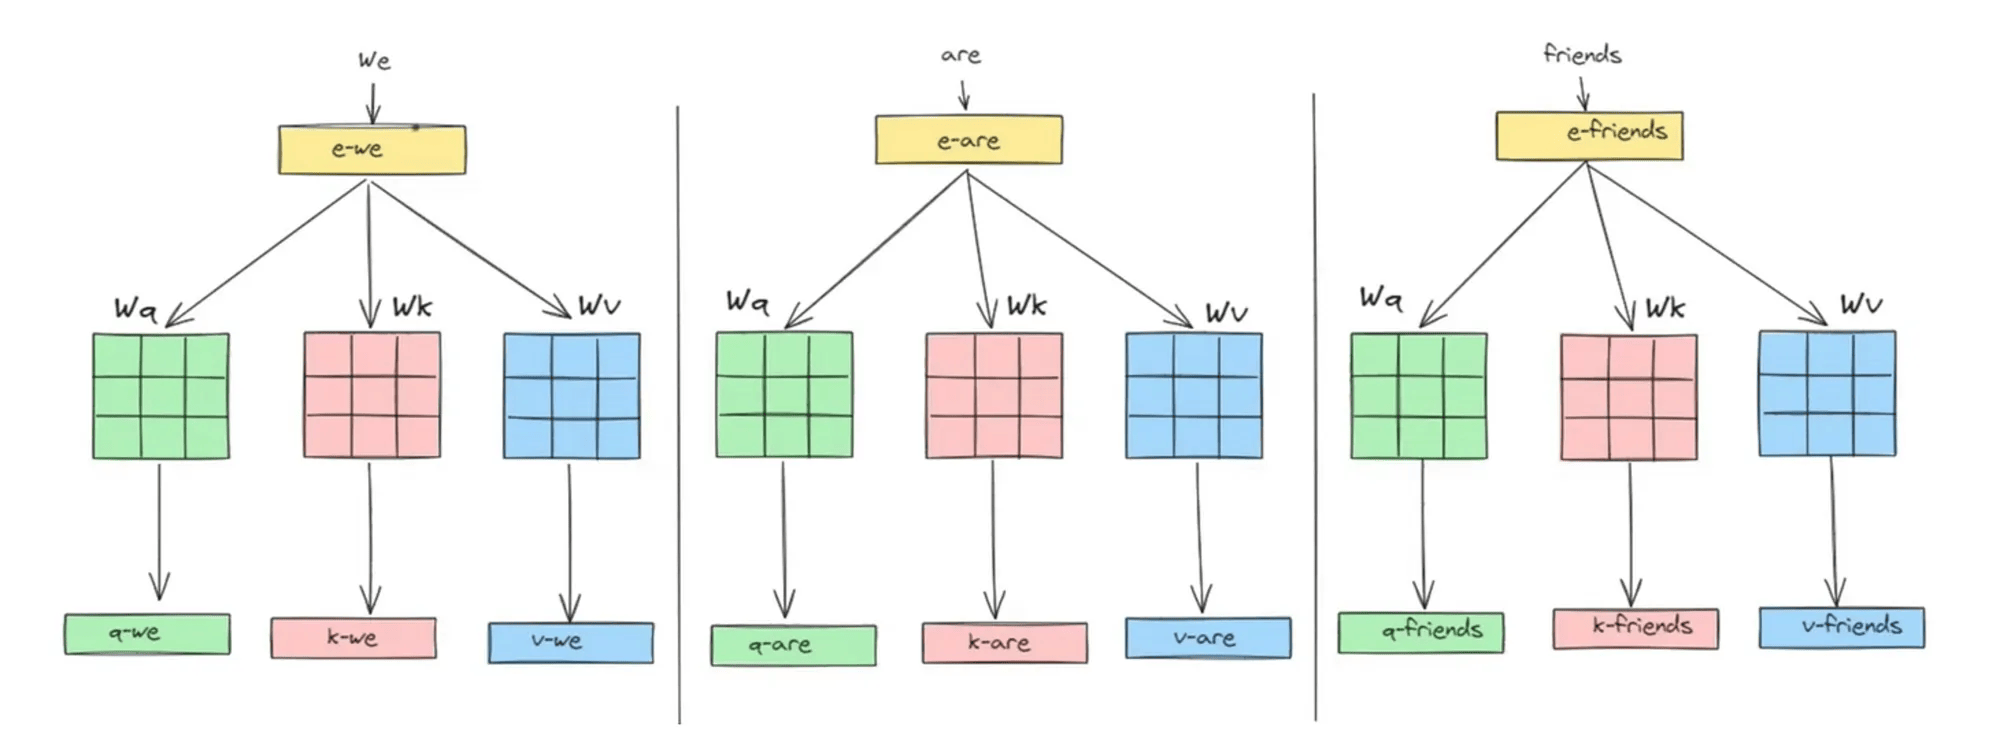
\includegraphics[width=0.8\linewidth]{Cross-Attention/processing-self-attention.png}
    \caption{Processing in self-attention}
\end{figure}

\begin{figure}[H]
    \centering
    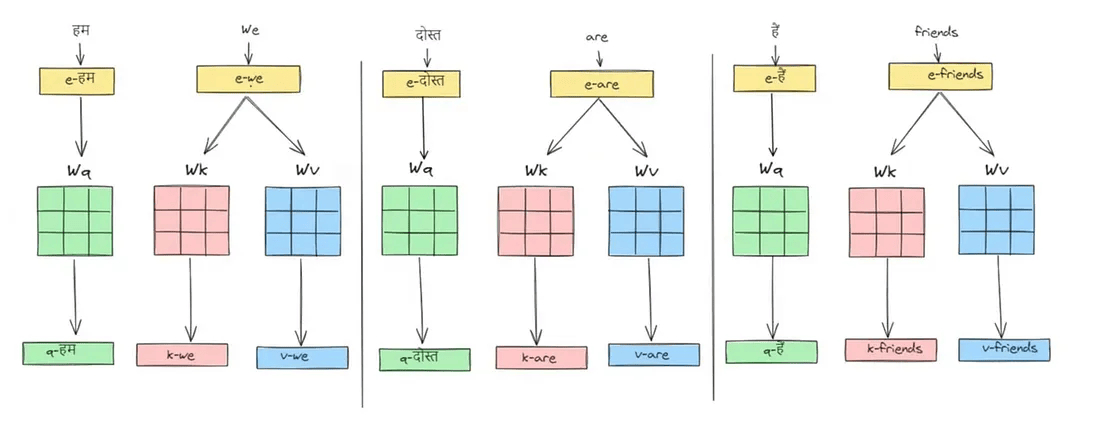
\includegraphics[width=0.8\linewidth]{Cross-Attention/processing-cross-attention.png}
    \caption{Processing in cross-attention}
\end{figure}

Just like self-attention, cross-attention calculates similarity scores between the query vectors from the output sequence and the key vectors from the input sequence. These scores are then used to weight the value vectors from the input sequence.

% Output of cross-attention
\section{The output}

In self-attention, we calculate the contextual embedding of each word of the input sequence as follows (values are randomly assigned):
\begin{align}
    \mathrm{ce}_{\mathrm{we}}
    &=
    0.8\,e_{\mathrm{we}}
    +
    0.1\,e_{\mathrm{are}}
    +
    0.1\,e_{\mathrm{friends}}
    \\[1em]
    \mathrm{ce}_{\mathrm{are}}
    &=
    0.15\,e_{\mathrm{we}}
    +
    0.75\,e_{\mathrm{are}}
    +
    0.1\,e_{\mathrm{friends}}
    \\[1em]
    \mathrm{ce}_{\mathrm{friends}}
    &=
    0.2\,e_{\mathrm{we}}
    +
    0.1\,e_{\mathrm{are}}
    +
    0.7\,e_{\mathrm{friends}}
\end{align}

In cross-attention, we deal with two sequences. Just like in self-attention, we obtain contextual embeddings here as well, but the number of contextual embeddings corresponds to the number of words in the output sequence. For example, if the output sequence has three words, like {\devanagarifont “हम”}, {\devanagarifont “दोस्त,”}  and {\devanagarifont “हैं,”} we will receive 3 contextual embeddings: one for each word. These contextual embeddings are also calculated based on the contribution of each input embedding to the output:
\begin{align}
    \text{ce}_{\text{\devanagarifont हम}}
    &=
    0.5\,e_{\text{we}}
    +
    0.3\,e_{\text{are}}
    +
    0.2\,e_{\text{friends}}
    \\[1em]
    \text{ce}_{\text{\devanagarifont दोस्त}}
    &=
    0.2\,e_{\text{we}}
    +
    0.2\,e_{\text{are}}
    +
    0.6\,e_{\text{friends}}
    \\[1em]
    \text{ce}_{\text{\devanagarifont हैं}}
    &=
    0.3\,e_{\text{we}}
    +
    0.4\,e_{\text{are}}
    +
    0.3\,e_{\text{friends}}
\end{align}